
%% bare_conf.tex
%% V1.3
%% 2007/01/11
%% by Michael Shell
%% See:
%% http://www.michaelshell.org/
%% for current contact information.
%%
%% This is a skeleton file demonstrating the use of IEEEtran.cls
%% (requires IEEEtran.cls version 1.7 or later) with an IEEE conference paper.
%%
%% Support sites:
%% http://www.michaelshell.org/tex/ieeetran/
%% http://www.ctan.org/tex-archive/macros/latex/contrib/IEEEtran/
%% and
%% http://www.ieee.org/

%%*************************************************************************
%% Legal Notice:
%% This code is offered as-is without any warranty either expressed or
%% implied; without even the implied warranty of MERCHANTABILITY or
%% FITNESS FOR A PARTICULAR PURPOSE!
%% User assumes all risk.
%% In no event shall IEEE or any contributor to this code be liable for
%% any damages or losses, including, but not limited to, incidental,
%% consequential, or any other damages, resulting from the use or misuse
%% of any information contained here.
%%
%% All comments are the opinions of their respective authors and are not
%% necessarily endorsed by the IEEE.
%%
%% This work is distributed under the LaTeX Project Public License (LPPL)
%% ( http://www.latex-project.org/ ) version 1.3, and may be freely used,
%% distributed and modified. A copy of the LPPL, version 1.3, is included
%% in the base LaTeX documentation of all distributions of LaTeX released
%% 2003/12/01 or later.
%% Retain all contribution notices and credits.
%% ** Modified files should be clearly indicated as such, including  **
%% ** renaming them and changing author support contact information. **
%%
%% File list of work: IEEEtran.cls, IEEEtran_HOWTO.pdf, bare_adv.tex,
%%                    bare_conf.tex, bare_jrnl.tex, bare_jrnl_compsoc.tex
%%*************************************************************************

% *** Authors should verify (and, if needed, correct) their LaTeX system  ***
% *** with the testflow diagnostic prior to trusting their LaTeX platform ***
% *** with production work. IEEE's font choices can trigger bugs that do  ***
% *** not appear when using other class files.                            ***
% The testflow support page is at:
% http://www.michaelshell.org/tex/testflow/



% Note that the a4paper option is mainly intended so that authors in
% countries using A4 can easily print to A4 and see how their papers will
% look in print - the typesetting of the document will not typically be
% affected with changes in paper size (but the bottom and side margins will).
% Use the testflow package mentioned above to verify correct handling of
% both paper sizes by the user's LaTeX system.
%
% Also note that the "draftcls" or "draftclsnofoot", not "draft", option
% should be used if it is desired that the figures are to be displayed in
% draft mode.
%
\documentclass[conference]{IEEEtran}
\usepackage{blindtext, graphicx}
% Add the compsoc option for Computer Society conferences.
%
% If IEEEtran.cls has not been installed into the LaTeX system files,
% manually specify the path to it like:
% \documentclass[conference]{../sty/IEEEtran}

\usepackage{color}



% Some very useful LaTeX packages include:
% (uncomment the ones you want to load)


% *** MISC UTILITY PACKAGES ***
%
%\usepackage{ifpdf}
% Heiko Oberdiek's ifpdf.sty is very useful if you need conditional
% compilation based on whether the output is pdf or dvi.
% usage:
% \ifpdf
%   % pdf code
% \else
%   % dvi code
% \fi
% The latest version of ifpdf.sty can be obtained from:
% http://www.ctan.org/tex-archive/macros/latex/contrib/oberdiek/
% Also, note that IEEEtran.cls V1.7 and later provides a builtin
% \ifCLASSINFOpdf conditional that works the same way.
% When switching from latex to pdflatex and vice-versa, the compiler may
% have to be run twice to clear warning/error messages.






% *** CITATION PACKAGES ***
%
%\usepackage{cite}
% cite.sty was written by Donald Arseneau
% V1.6 and later of IEEEtran pre-defines the format of the cite.sty package
% \cite{} output to follow that of IEEE. Loading the cite package will
% result in citation numbers being automatically sorted and properly
% "compressed/ranged". e.g., [1], [9], [2], [7], [5], [6] without using
% cite.sty will become [1], [2], [5]--[7], [9] using cite.sty. cite.sty's
% \cite will automatically add leading space, if needed. Use cite.sty's
% noadjust option (cite.sty V3.8 and later) if you want to turn this off.
% cite.sty is already installed on most LaTeX systems. Be sure and use
% version 4.0 (2003-05-27) and later if using hyperref.sty. cite.sty does
% not currently provide for hyperlinked citations.
% The latest version can be obtained at:
% http://www.ctan.org/tex-archive/macros/latex/contrib/cite/
% The documentation is contained in the cite.sty file itself.






% *** GRAPHICS RELATED PACKAGES ***
%
\ifCLASSINFOpdf
  % \usepackage[pdftex]{graphicx}
  % declare the path(s) where your graphic files are
  % \graphicspath{{../pdf/}{../jpeg/}}
  % and their extensions so you won't have to specify these with
  % every instance of \includegraphics
  % \DeclareGraphicsExtensions{.pdf,.jpeg,.png}
\else
  % or other class option (dvipsone, dvipdf, if not using dvips). graphicx
  % will default to the driver specified in the system graphics.cfg if no
  % driver is specified.
  % \usepackage[dvips]{graphicx}
  % declare the path(s) where your graphic files are
  % \graphicspath{{../eps/}}
  % and their extensions so you won't have to specify these with
  % every instance of \includegraphics
  % \DeclareGraphicsExtensions{.eps}
\fi
% graphicx was written by David Carlisle and Sebastian Rahtz. It is
% required if you want graphics, photos, etc. graphicx.sty is already
% installed on most LaTeX systems. The latest version and documentation can
% be obtained at:
% http://www.ctan.org/tex-archive/macros/latex/required/graphics/
% Another good source of documentation is "Using Imported Graphics in
% LaTeX2e" by Keith Reckdahl which can be found as epslatex.ps or
% epslatex.pdf at: http://www.ctan.org/tex-archive/info/
%
% latex, and pdflatex in dvi mode, support graphics in encapsulated
% postscript (.eps) format. pdflatex in pdf mode supports graphics
% in .pdf, .jpeg, .png and .mps (metapost) formats. Users should ensure
% that all non-photo figures use a vector format (.eps, .pdf, .mps) and
% not a bitmapped formats (.jpeg, .png). IEEE frowns on bitmapped formats
% which can result in "jaggedy"/blurry rendering of lines and letters as
% well as large increases in file sizes.
%
% You can find documentation about the pdfTeX application at:
% http://www.tug.org/applications/pdftex





% *** MATH PACKAGES ***
%
%\usepackage[cmex10]{amsmath}
% A popular package from the American Mathematical Society that provides
% many useful and powerful commands for dealing with mathematics. If using
% it, be sure to load this package with the cmex10 option to ensure that
% only type 1 fonts will utilized at all point sizes. Without this option,
% it is possible that some math symbols, particularly those within
% footnotes, will be rendered in bitmap form which will result in a
% document that can not be IEEE Xplore compliant!
%
% Also, note that the amsmath package sets \interdisplaylinepenalty to 10000
% thus preventing page breaks from occurring within multiline equations. Use:
%\interdisplaylinepenalty=2500
% after loading amsmath to restore such page breaks as IEEEtran.cls normally
% does. amsmath.sty is already installed on most LaTeX systems. The latest
% version and documentation can be obtained at:
% http://www.ctan.org/tex-archive/macros/latex/required/amslatex/math/





% *** SPECIALIZED LIST PACKAGES ***
%
%\usepackage{algorithmic}
% algorithmic.sty was written by Peter Williams and Rogerio Brito.
% This package provides an algorithmic environment fo describing algorithms.
% You can use the algorithmic environment in-text or within a figure
% environment to provide for a floating algorithm. Do NOT use the algorithm
% floating environment provided by algorithm.sty (by the same authors) or
% algorithm2e.sty (by Christophe Fiorio) as IEEE does not use dedicated
% algorithm float types and packages that provide these will not provide
% correct IEEE style captions. The latest version and documentation of
% algorithmic.sty can be obtained at:
% http://www.ctan.org/tex-archive/macros/latex/contrib/algorithms/
% There is also a support site at:
% http://algorithms.berlios.de/index.html
% Also of interest may be the (relatively newer and more customizable)
% algorithmicx.sty package by Szasz Janos:
% http://www.ctan.org/tex-archive/macros/latex/contrib/algorithmicx/




% *** ALIGNMENT PACKAGES ***
%
%\usepackage{array}
% Frank Mittelbach's and David Carlisle's array.sty patches and improves
% the standard LaTeX2e array and tabular environments to provide better
% appearance and additional user controls. As the default LaTeX2e table
% generation code is lacking to the point of almost being broken with
% respect to the quality of the end results, all users are strongly
% advised to use an enhanced (at the very least that provided by array.sty)
% set of table tools. array.sty is already installed on most systems. The
% latest version and documentation can be obtained at:
% http://www.ctan.org/tex-archive/macros/latex/required/tools/


%\usepackage{mdwmath}
%\usepackage{mdwtab}
% Also highly recommended is Mark Wooding's extremely powerful MDW tools,
% especially mdwmath.sty and mdwtab.sty which are used to format equations
% and tables, respectively. The MDWtools set is already installed on most
% LaTeX systems. The lastest version and documentation is available at:
% http://www.ctan.org/tex-archive/macros/latex/contrib/mdwtools/


% IEEEtran contains the IEEEeqnarray family of commands that can be used to
% generate multiline equations as well as matrices, tables, etc., of high
% quality.


%\usepackage{eqparbox}
% Also of notable interest is Scott Pakin's eqparbox package for creating
% (automatically sized) equal width boxes - aka "natural width parboxes".
% Available at:
% http://www.ctan.org/tex-archive/macros/latex/contrib/eqparbox/





% *** SUBFIGURE PACKAGES ***
%\usepackage[tight,footnotesize]{subfigure}
% subfigure.sty was written by Steven Douglas Cochran. This package makes it
% easy to put subfigures in your figures. e.g., "Figure 1a and 1b". For IEEE
% work, it is a good idea to load it with the tight package option to reduce
% the amount of white space around the subfigures. subfigure.sty is already
% installed on most LaTeX systems. The latest version and documentation can
% be obtained at:
% http://www.ctan.org/tex-archive/obsolete/macros/latex/contrib/subfigure/
% subfigure.sty has been superceeded by subfig.sty.



%\usepackage[caption=false]{caption}
%\usepackage[font=footnotesize]{subfig}
% subfig.sty, also written by Steven Douglas Cochran, is the modern
% replacement for subfigure.sty. However, subfig.sty requires and
% automatically loads Axel Sommerfeldt's caption.sty which will override
% IEEEtran.cls handling of captions and this will result in nonIEEE style
% figure/table captions. To prevent this problem, be sure and preload
% caption.sty with its "caption=false" package option. This is will preserve
% IEEEtran.cls handing of captions. Version 1.3 (2005/06/28) and later
% (recommended due to many improvements over 1.2) of subfig.sty supports
% the caption=false option directly:
%\usepackage[caption=false,font=footnotesize]{subfig}
%
% The latest version and documentation can be obtained at:
% http://www.ctan.org/tex-archive/macros/latex/contrib/subfig/
% The latest version and documentation of caption.sty can be obtained at:
% http://www.ctan.org/tex-archive/macros/latex/contrib/caption/




% *** FLOAT PACKAGES ***
%
%\usepackage{fixltx2e}
% fixltx2e, the successor to the earlier fix2col.sty, was written by
% Frank Mittelbach and David Carlisle. This package corrects a few problems
% in the LaTeX2e kernel, the most notable of which is that in current
% LaTeX2e releases, the ordering of single and double column floats is not
% guaranteed to be preserved. Thus, an unpatched LaTeX2e can allow a
% single column figure to be placed prior to an earlier double column
% figure. The latest version and documentation can be found at:
% http://www.ctan.org/tex-archive/macros/latex/base/



%\usepackage{stfloats}
% stfloats.sty was written by Sigitas Tolusis. This package gives LaTeX2e
% the ability to do double column floats at the bottom of the page as well
% as the top. (e.g., "\begin{figure*}[!b]" is not normally possible in
% LaTeX2e). It also provides a command:
%\fnbelowfloat
% to enable the placement of footnotes below bottom floats (the standard
% LaTeX2e kernel puts them above bottom floats). This is an invasive package
% which rewrites many portions of the LaTeX2e float routines. It may not work
% with other packages that modify the LaTeX2e float routines. The latest
% version and documentation can be obtained at:
% http://www.ctan.org/tex-archive/macros/latex/contrib/sttools/
% Documentation is contained in the stfloats.sty comments as well as in the
% presfull.pdf file. Do not use the stfloats baselinefloat ability as IEEE
% does not allow \baselineskip to stretch. Authors submitting work to the
% IEEE should note that IEEE rarely uses double column equations and
% that authors should try to avoid such use. Do not be tempted to use the
% cuted.sty or midfloat.sty packages (also by Sigitas Tolusis) as IEEE does
% not format its papers in such ways.





% *** PDF, URL AND HYPERLINK PACKAGES ***
%
%\usepackage{url}
% url.sty was written by Donald Arseneau. It provides better support for
% handling and breaking URLs. url.sty is already installed on most LaTeX
% systems. The latest version can be obtained at:
% http://www.ctan.org/tex-archive/macros/latex/contrib/misc/
% Read the url.sty source comments for usage information. Basically,
% \url{my_url_here}.





% *** Do not adjust lengths that control margins, column widths, etc. ***
% *** Do not use packages that alter fonts (such as pslatex).         ***
% There should be no need to do such things with IEEEtran.cls V1.6 and later.
% (Unless specifically asked to do so by the journal or conference you plan
% to submit to, of course. )


% correct bad hyphenation here
\hyphenation{op-tical net-works semi-conduc-tor}


\begin{document}
%
% paper title
% can use linebreaks \\ within to get better formatting as desired
\title{DQM4HEP : A generic\\Data Quality Monitoring for High Energy Physics}


% author names and affiliations
% use a multiple column layout for up to three different
% affiliations

\author{

\IEEEauthorblockN{R\'emi \'Et\'e}
\IEEEauthorblockA{Univ, Lyon, Universit\'e Lyon 1, \\
CNRS/IN2P3, IPNL 4 rue E Fermi \\
69622, Villeurbanne CEDEX, France\\
Email: rete@ipnl.in2p3.fr}

\and

\IEEEauthorblockN{Antoine Pingault}
\IEEEauthorblockA{Ghent University, Department of Physics \\
and Astronomy Proeftuinstraat 86,\\
B-9000 Gent, Belgium\\
Email: antoine.pingault@ugent.be}

\and

\IEEEauthorblockN{Laurent Mirabito}
\IEEEauthorblockA{Univ, Lyon, Universit\'e Lyon 1, \\
CNRS/IN2P3, IPNL 4 rue E Fermi \\
69622, Villeurbanne CEDEX, France\\
Email: mirabito@ipnl.in2p3.fr}

}


% conference papers do not typically use \thanks and this command
% is locked out in conference mode. If really needed, such as for
% the acknowledgment of grants, issue a \IEEEoverridecommandlockouts
% after \documentclass

% for over three affiliations, or if they all won't fit within the width
% of the page, use this alternative format:
%
%\author{\IEEEauthorblockN{Michael Shell\IEEEauthorrefmark{1},
%Homer Simpson\IEEEauthorrefmark{2},
%James Kirk\IEEEauthorrefmark{3},
%Montgomery Scott\IEEEauthorrefmark{3} and
%Eldon Tyrell\IEEEauthorrefmark{4}}
%\IEEEauthorblockA{\IEEEauthorrefmark{1}School of Electrical and Computer Engineering\\
%Georgia Institute of Technology,
%Atlanta, Georgia 30332--0250\\ Email: see http://www.michaelshell.org/contact.html}
%\IEEEauthorblockA{\IEEEauthorrefmark{2}Twentieth Century Fox, Springfield, USA\\
%Email: homer@thesimpsons.com}
%\IEEEauthorblockA{\IEEEauthorrefmark{3}Starfleet Academy, San Francisco, California 96678-2391\\
%Telephone: (800) 555--1212, Fax: (888) 555--1212}
%\IEEEauthorblockA{\IEEEauthorrefmark{4}Tyrell Inc., 123 Replicant Street, Los Angeles, California 90210--4321}}




% use for special paper notices
%\IEEEspecialpapernotice{(Invited Paper)}




% make the title area
\maketitle


\begin{abstract}
With increasingly sophisticated experiment, online Data Quality Monitoring (DQM) is of a significant importance for the detector and operation efficiency. Most experiments developed and built a dedicated monitoring system on top of their Event Data Model (EDM). This leads to a strong dependency to the data format and storage, making the reusability of the system for another experiment difficult. To increase the flexibility and porting of software across experiments, a generic online Data Quality Monitoring system has been developed without any assumption on the Event Data Model and data type to treat. The aim here, is to provide reusable and flexible tools for scientists to monitor their detectors by focusing on the analysis part.

In addition, a dedicated implementation, based on the LCIO~\cite{LCIO} Event Data Model for the Linear Collider Collaboration (LCC), was also developed. It has already been put to real condition testing during test beam campaigns at CERN\footnote{Conseil Européen pour la Recherche Nucléaire} with a combined detector setup composed of the CALICE\footnote{CAlorimeter for LInear Collider Experiment} Semi-Digital Hadronic CALorimeter (SDHCAL) and Silicon Tungsten Electronic Calorimeter (SiWECal) prototypes.
\end{abstract}
% IEEEtran.cls defaults to using nonbold math in the Abstract.
% This preserves the distinction between vectors and scalars. However,
% if the journal you are submitting to favors bold math in the abstract,
% then you can use LaTeX's standard command \boldmath at the very start
% of the abstract to achieve this. Many IEEE journals frown on math
% in the abstract anyway.

% Note that keywords are not normally used for peerreview papers.
\begin{IEEEkeywords}
DQM, High Energy Physics, Detector, DAQ.
\end{IEEEkeywords}






% For peer review papers, you can put extra information on the cover
% page as needed:
% \ifCLASSOPTIONpeerreview
% \begin{center} \bfseries EDICS Category: 3-BBND \end{center}
% \fi
%
% For peerreview papers, this IEEEtran command inserts a page break and
% creates the second title. It will be ignored for other modes.
\IEEEpeerreviewmaketitle


%~~~~~~~~~~~~~~~~~~~~~~~~~%
%~~~~~~~~~~~~~~~~~~~~~~~~~%

\section{Introduction}
The purpose of a monitoring system is to help identify problems when the experiment is running. For this, it needs to fulfil two requirements : it must display a quick overview of the status and working order of every detector part and should also evaluate the quality of the data being taken. This implies some key infrastructure points for the monitoring software. First, as it should be running at all times when taking data, it needs to interface with the Data Acquisition (DAQ) system. It must not however interfere with the data taking process (slow down, stop, etc.). It needs a system to distribute data coming from the DAQ to the analysis tools and then to visualization tools. The data analysis and data quality assessment needs to remain user-defined and visualization interfaces accessible from many client PCs.

In computer science, generic programming implies an architecture with algorithms independent of a programming data type. Algorithms can be instantiated when needed, and in different ways to work with multiple data representations. This leads to more flexible and easily reusable software.

The genericity of the framework that is presented here, lies in two core features: its Event Data Model (EDM) abstraction and plugin system.

The EDM abstraction gives the ability to the user to define the type of event to use together with its serialization process. The plugin system, permits the inclusion of any user classes via external libraries. One can use plugin abstraction and factories to select the serialization process, online analysis, etc.

The framework is also designed to run each applications as an independent process. They are linked to each other by network communications with either TCP/IP or HTTP protocols using DIM~\cite{DIM} and Mongoose~\cite{MONGOOSE} respectively. This helps distributing the load from the processes over the multiple cores and computers.

To implement this solution for its own experiment, an user has to define the event type to treat and its serialization. An interface, \textit{xdrstream}, is provided within the framework to simplify the later.


%~~~~~~~~~~~~~~~~~~~~~~~~~~~~~~~~~~~~~~~~~~~~~~~~~~~~~~~~~~~~~~~~%
%~~~~~~~~~~~~~~~~~~~~~~~~~~~~~~~~~~~~~~~~~~~~~~~~~~~~~~~~~~~~~~~~%
\section{Software architecture}
{\color{red}Some intro}

Overall framework architecture is displayed on Fig.~\ref{fig:DQM4HEPArchitecture}
\begin{figure}[htbp]
  \begin{center}
    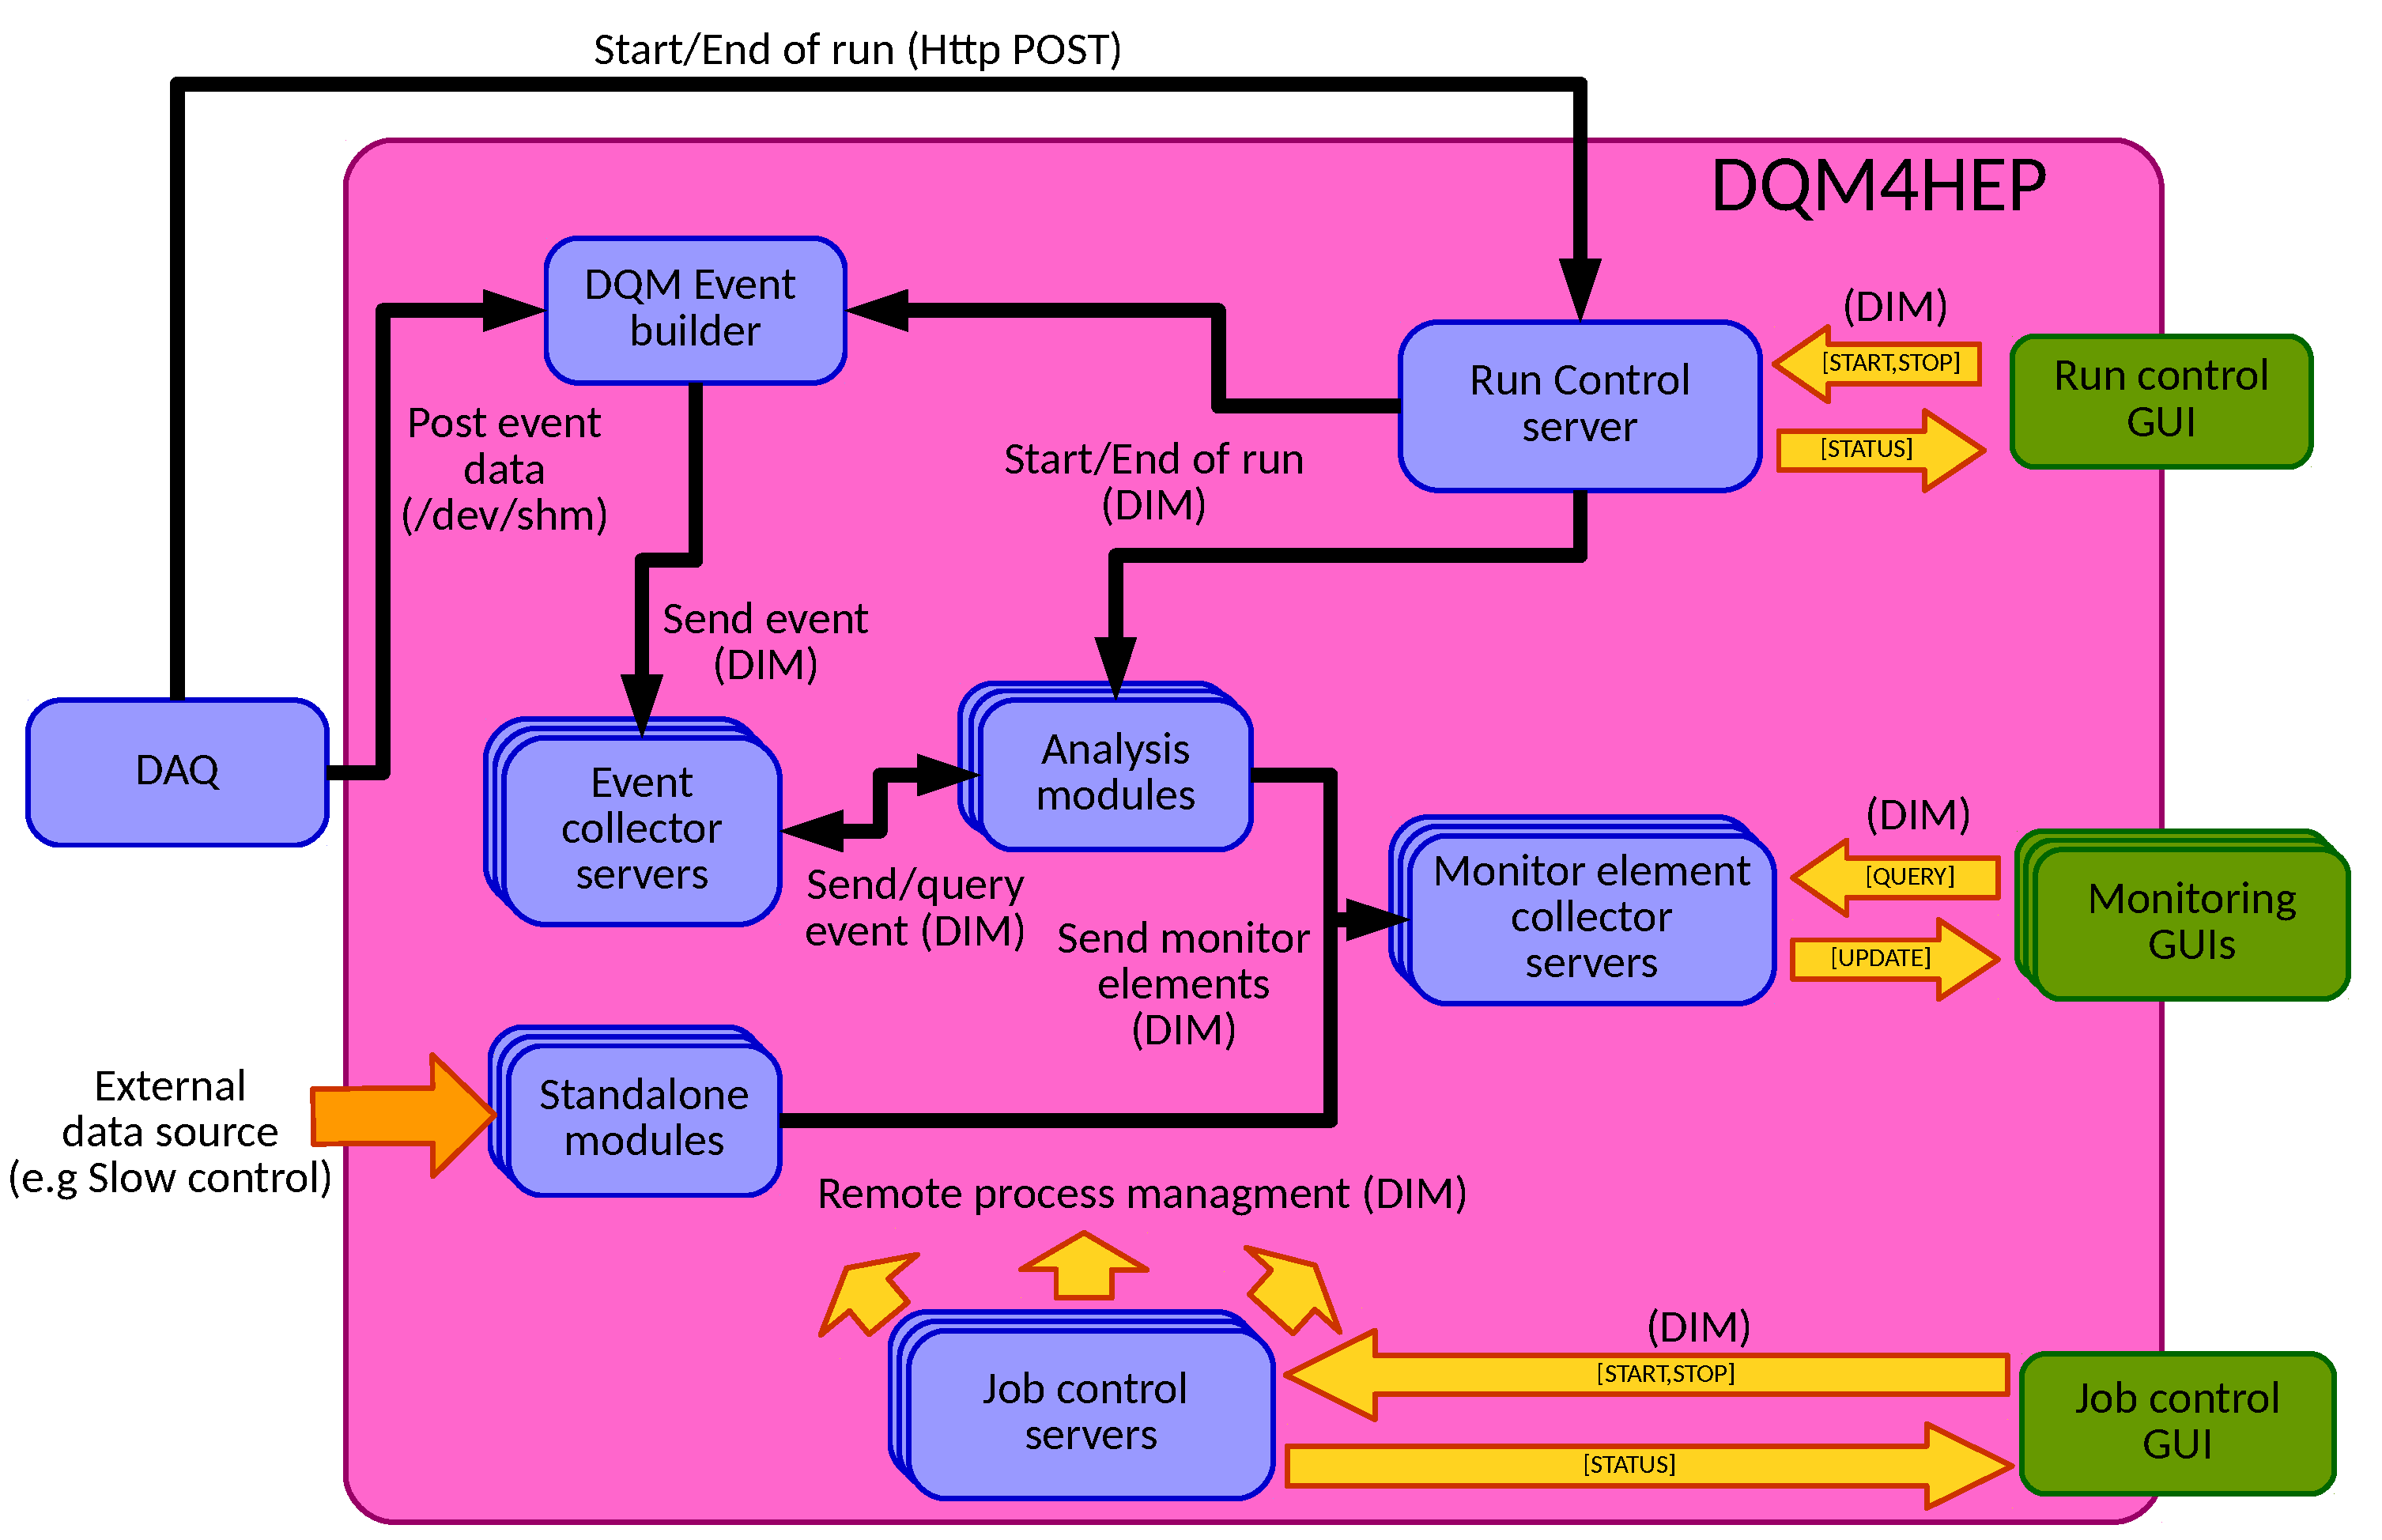
\includegraphics[width=0.95\linewidth]{figs/GlobalArchitectureDiagram.pdf}
    \caption{\label{fig:DQM4HEPArchitecture} DQM4HEP framework architecture}
  \end{center}
\end{figure}


%~~~~~~~~~~~~~~~~~~~~~~~~~~~~~~~~~~~~~~~~~~~~~~~~~~~~~~~~~~~~~~~~%
\subsection{Link to DAQ system}
As explained before, to efficiently run an experiment the monitoring system and the DAQ system needs to be somewhat linked. To control the data acquisition, the DAQ system sends start/stop/status signals to the read out electronics of the detectors. The monitoring system can be set up to receive such signals by
its \textit{Run Control Server} before dispatching it to the DQM applications. Thus, starting (stopping) a new run from the DAQ system will automatically start (stop) the DQM applications.

Second coupling to the DAQ system is the \textit{event builder} as depicted in Fig.~\ref{fig:DQMEventBuilder}. Its purposes is to get the raw data collected by the DAQ system (e.g. from a shared memory space) and convert it to an user defined data structure using plugins called \textit{processors}. The reconstructed events are then serialized and sent to event collectors over the network.

\begin{figure}[htbp]
  \begin{center}
    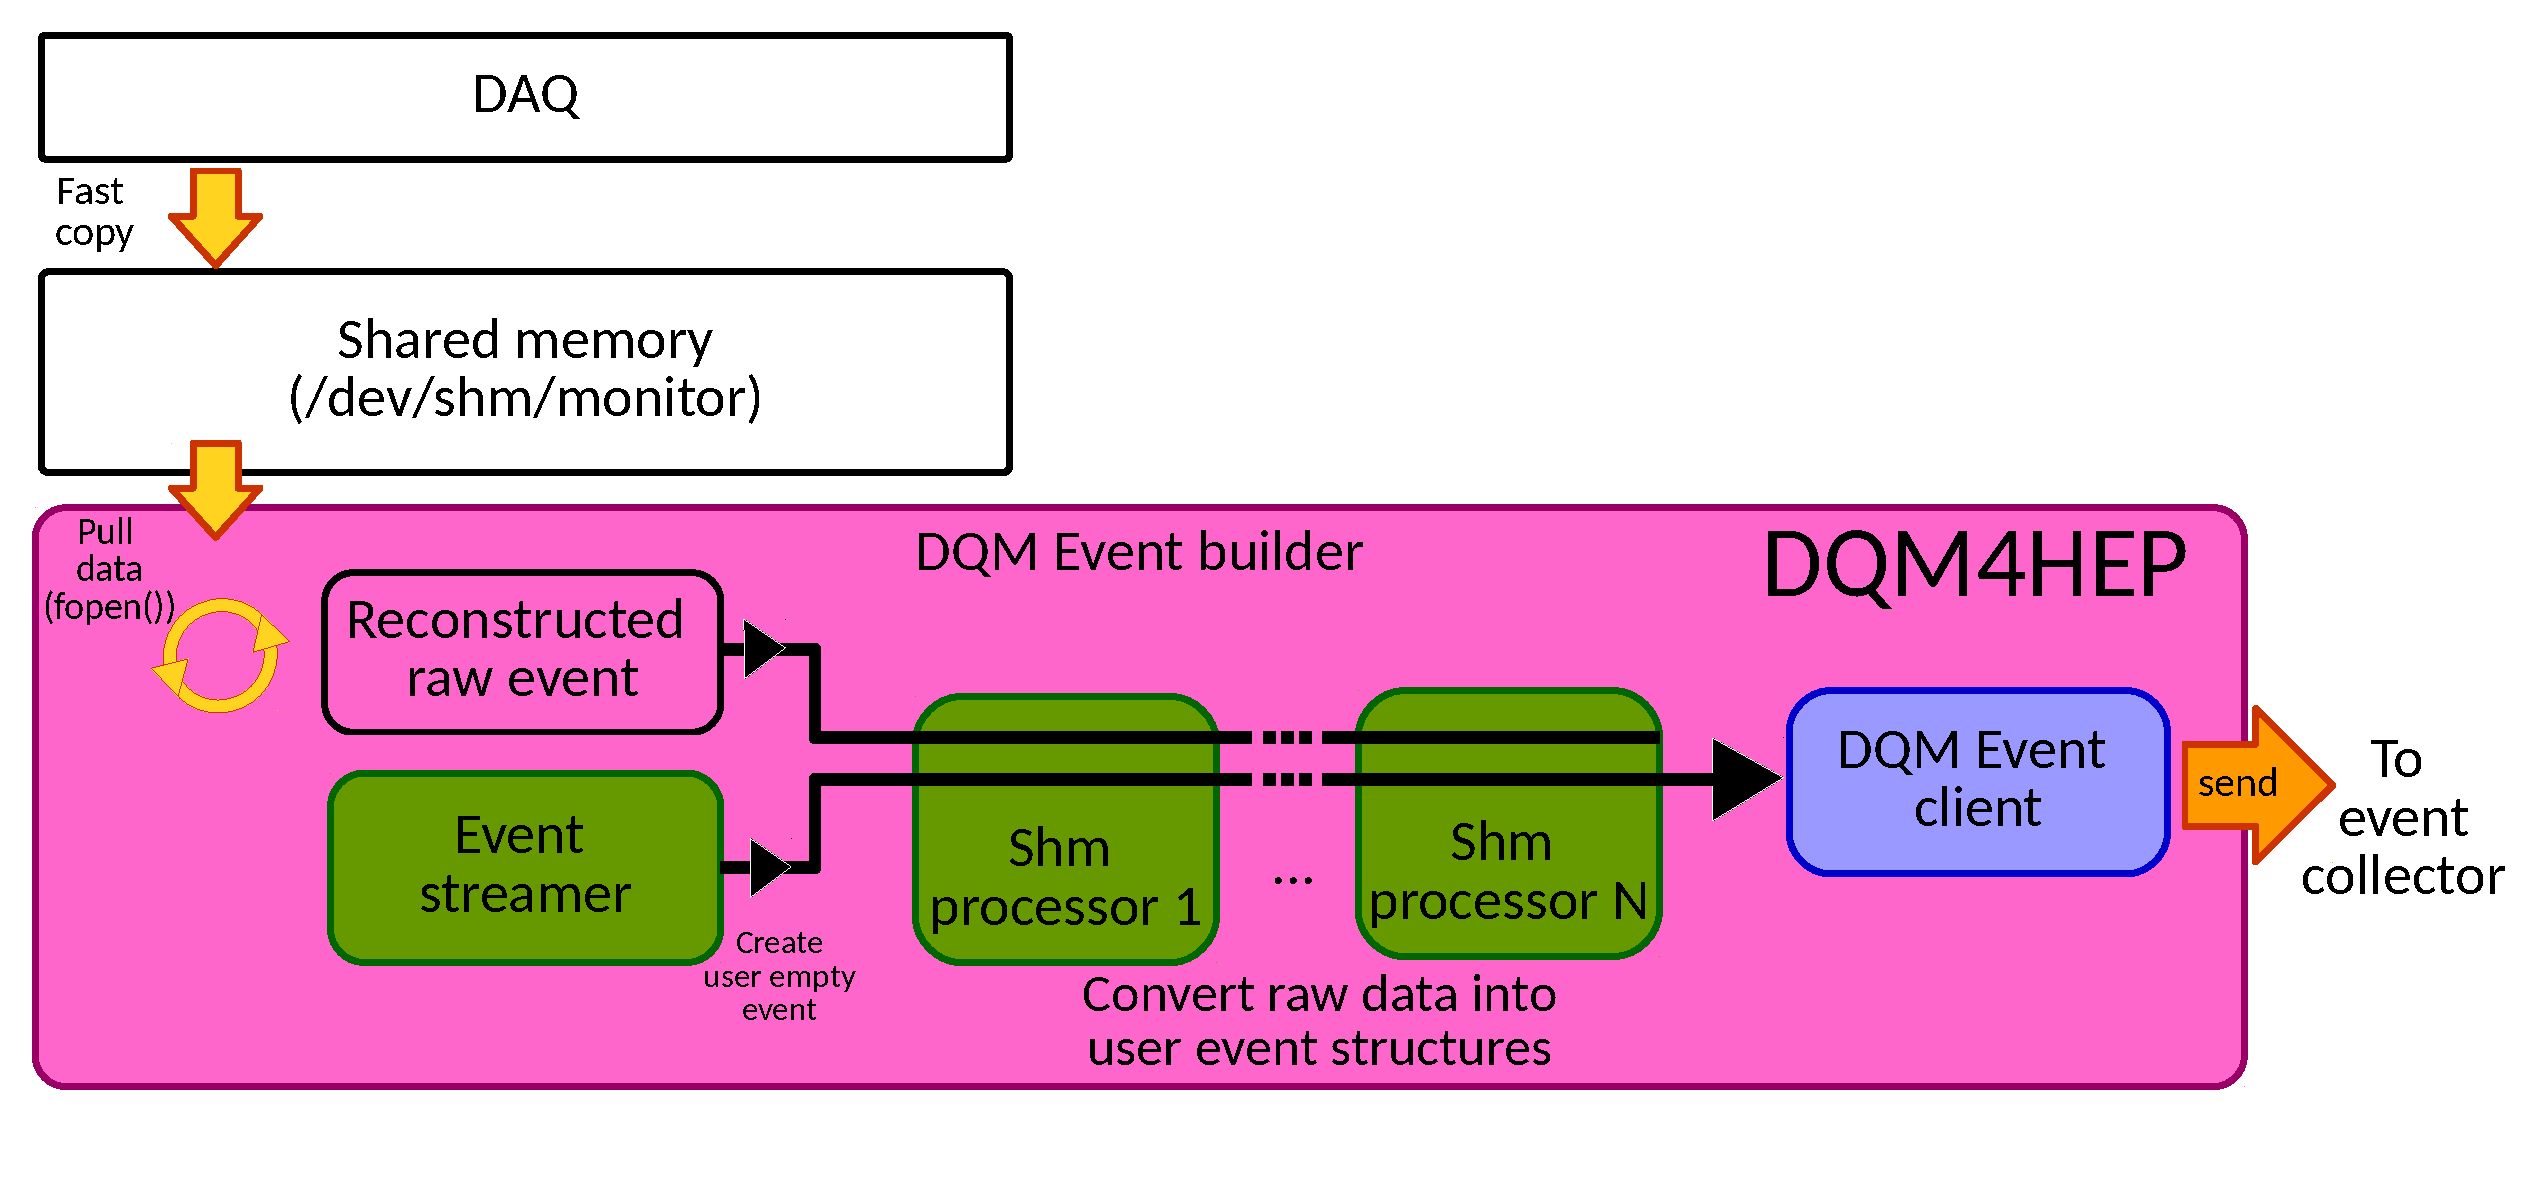
\includegraphics[width=0.95\linewidth]{figs/EventBuilderDiagram_IEEE.pdf}
    \caption{\label{fig:DQMEventBuilder} Sketch of the event building process within the framework.}
  \end{center}
\end{figure}

It should be emphasized here that this is the only coupling to the DAQ system, and so represents the only work required from the DAQ engineer to couple the framework with an experiment.


%~~~~~~~~~~~~~~~~~~~~~~~~~~~~~~~~~~~~~~~~~~~~~~~~~~~~~~~~~~~~~~~~%
\subsection{Collectors}
With the ability of balancing the load over multiple cores and computers comes the need of a common access point for data. Two types of applications serve this process in the framework. The \textit{event collector} acts as the bridge between the event builder and the various analysis modules. The \textit{monitor element collector} share the same role between the analysis modules and the visualization interfaces.

As it can be seen on Fig.~\ref{fig:DQMDataAccess}, data from these collectors can then be accessed either via direct user query (i.e. modules send a query to the collector to receive the last recorded event) or via permanent subscription (modules are notified when a new event is collected).

To start such an application, only the collector name is needed. This name is passed using command line argument at start-up and will be used to identify the collector over the network for external applications.  

\begin{figure}[htbp]
  \begin{center}
    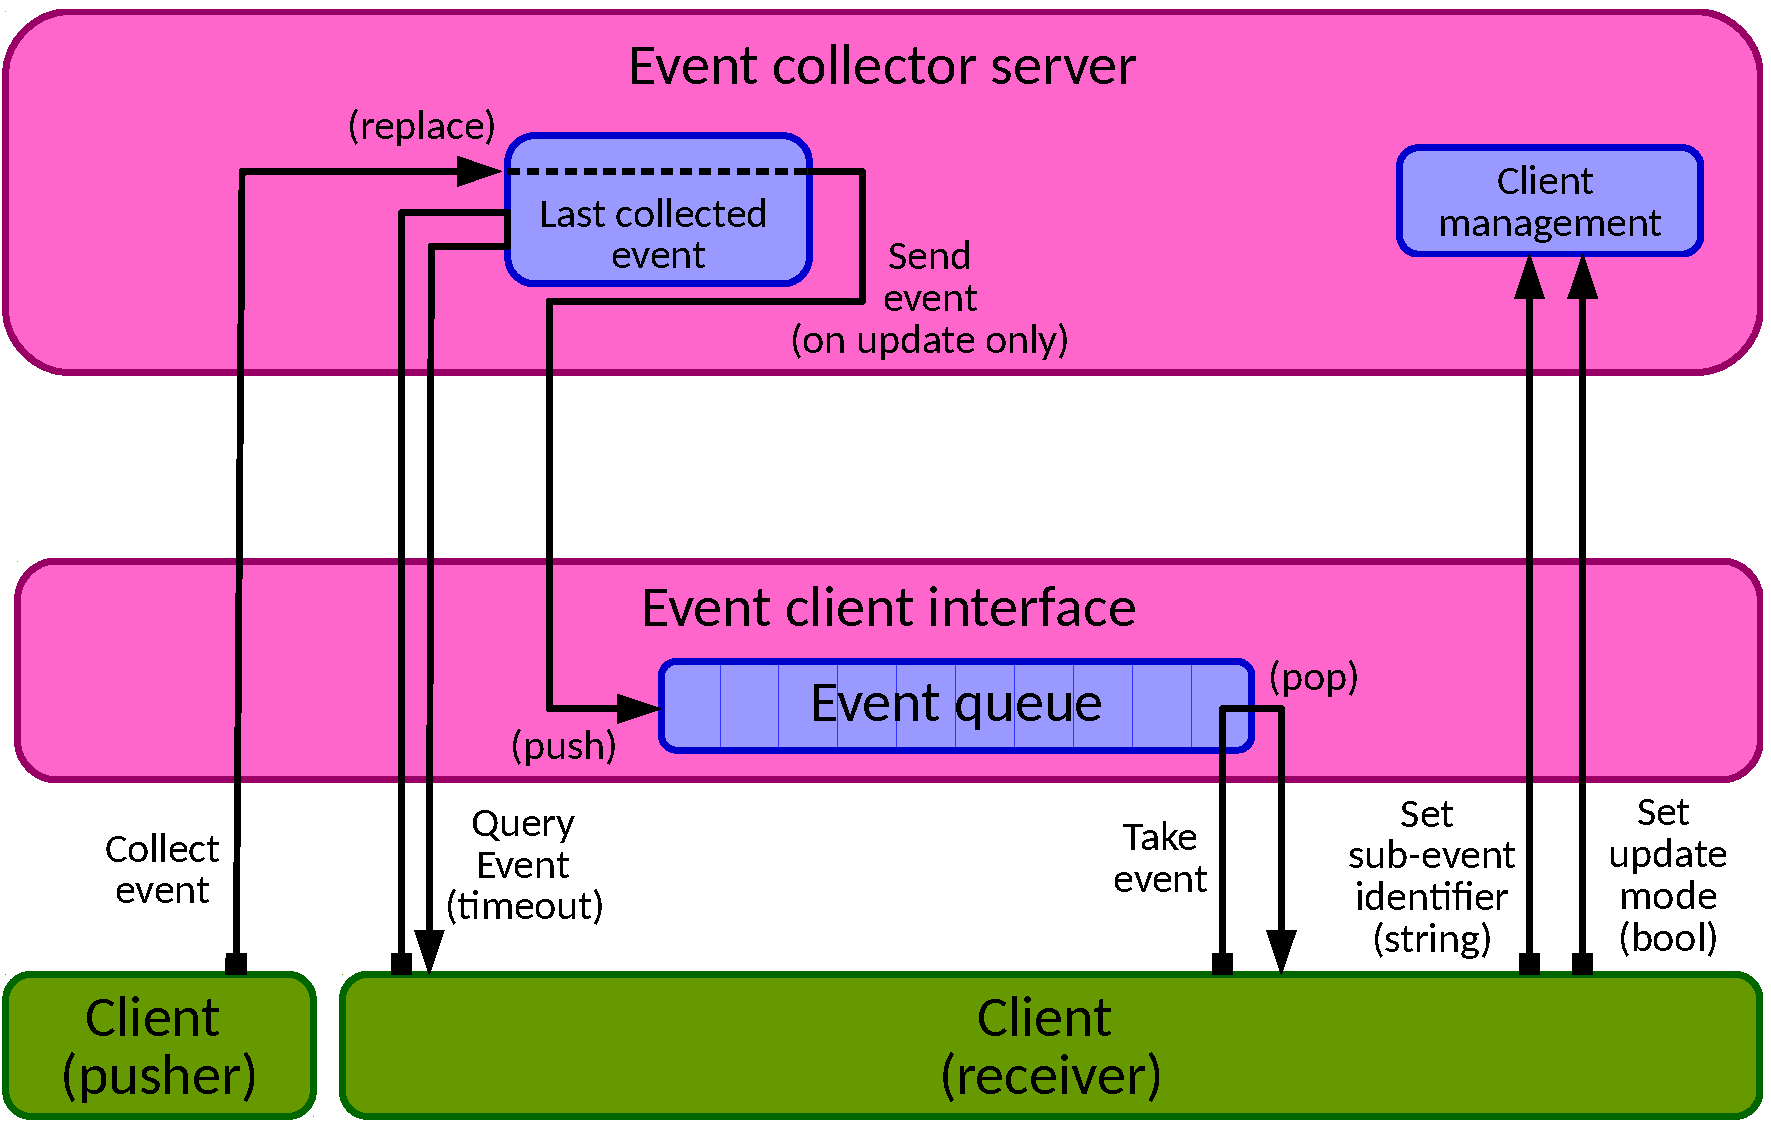
\includegraphics[width=0.95\linewidth]{figs/EventCollectorDiagram.pdf}
    \caption{\label{fig:DQMDataAccess} Schematic view of possible interactions between an event collector and a client application.}
  \end{center}
\end{figure}

%~~~~~~~~~~~~~~~~~~~~~~~~~~~~~~~~~~~~~~~~~~~~~~~~~~~~~~~~~~~~~~~~%
\subsection{Online data analysis}
Depending on the data input, two types of applications can be used within the framework. The first one, the analysis module, analyze reconstructed event from the event collectors and thus runs only while the DAQ is taking data. The second type, the standalone module, is independent of the DAQ status and use external data source defined by the user (e.g. environmental data stored in a database).

Both are implemented as user defined plug-ins and aim to analyze and reduce data to a few self-described objects called \emph{monitor elements}. These wrap graphics objects such as histogram or graph, plus some meta data about data quality or run-time information. 

On each monitor element can be run multiple quality tests used to assess the data quality. The quality test results are bound to the monitor elements and sent together to the collector so that user can then be alerted if quality reaches low/dangerous threshold (e.g. high current value, saturation in part of detector, etc.). If deemed necessary, user has the ability to archive monitor elements for off-line checks in ROOT files.

The overall framework architecture gives the flexibility to start (stop) any analysis modules at any given time, including during data taking. This important point means that adding, removing, modifying a module even while taking data will never interfere with DAQ system.

%~~~~~~~~~~~~~~~~~~~~~~~~~~~~~~~~~~~~~~~~~~~~~~~~~~~~~~~~~~~~~~~~%
\subsection{Cycle structure for data processing}

During an acquisition, data taking can be non continuous or with a high rate. For performance reason, there no need to send monitor elements after each processed event. In case of a high rate data taking, this also implies to refresh the visualization too frequently. For these reasons, data in online module application are processed during cycles, during which events are processed sequentially. At the end of cycle, the monitor element are sent to the collector and the visualization interfaces refreshed. Cycles are implemented as plug-ins so user can defined their own to suit their needs. The DQM4HEP framework provides three cycle implementations :

\begin{itemize}
  \item a \textit{timer cycle}, for which events are processed during \textit{n} seconds,
  \item an \textit{event counter cycle}, for which \textit{n} events are processed before ending,
  \item an \textit{event size cycle}, for which \textit{n} bytes of serialized data are processed before ending
\end{itemize}

Fig.~\ref{fig:DQMCycleSystem} shows the analysis module application workflow where the central part is dedicated to the cycle logic (\textit{start}/\textit{processEvent}/\textit{end}). 

\begin{figure}[htbp]
  \begin{center}
    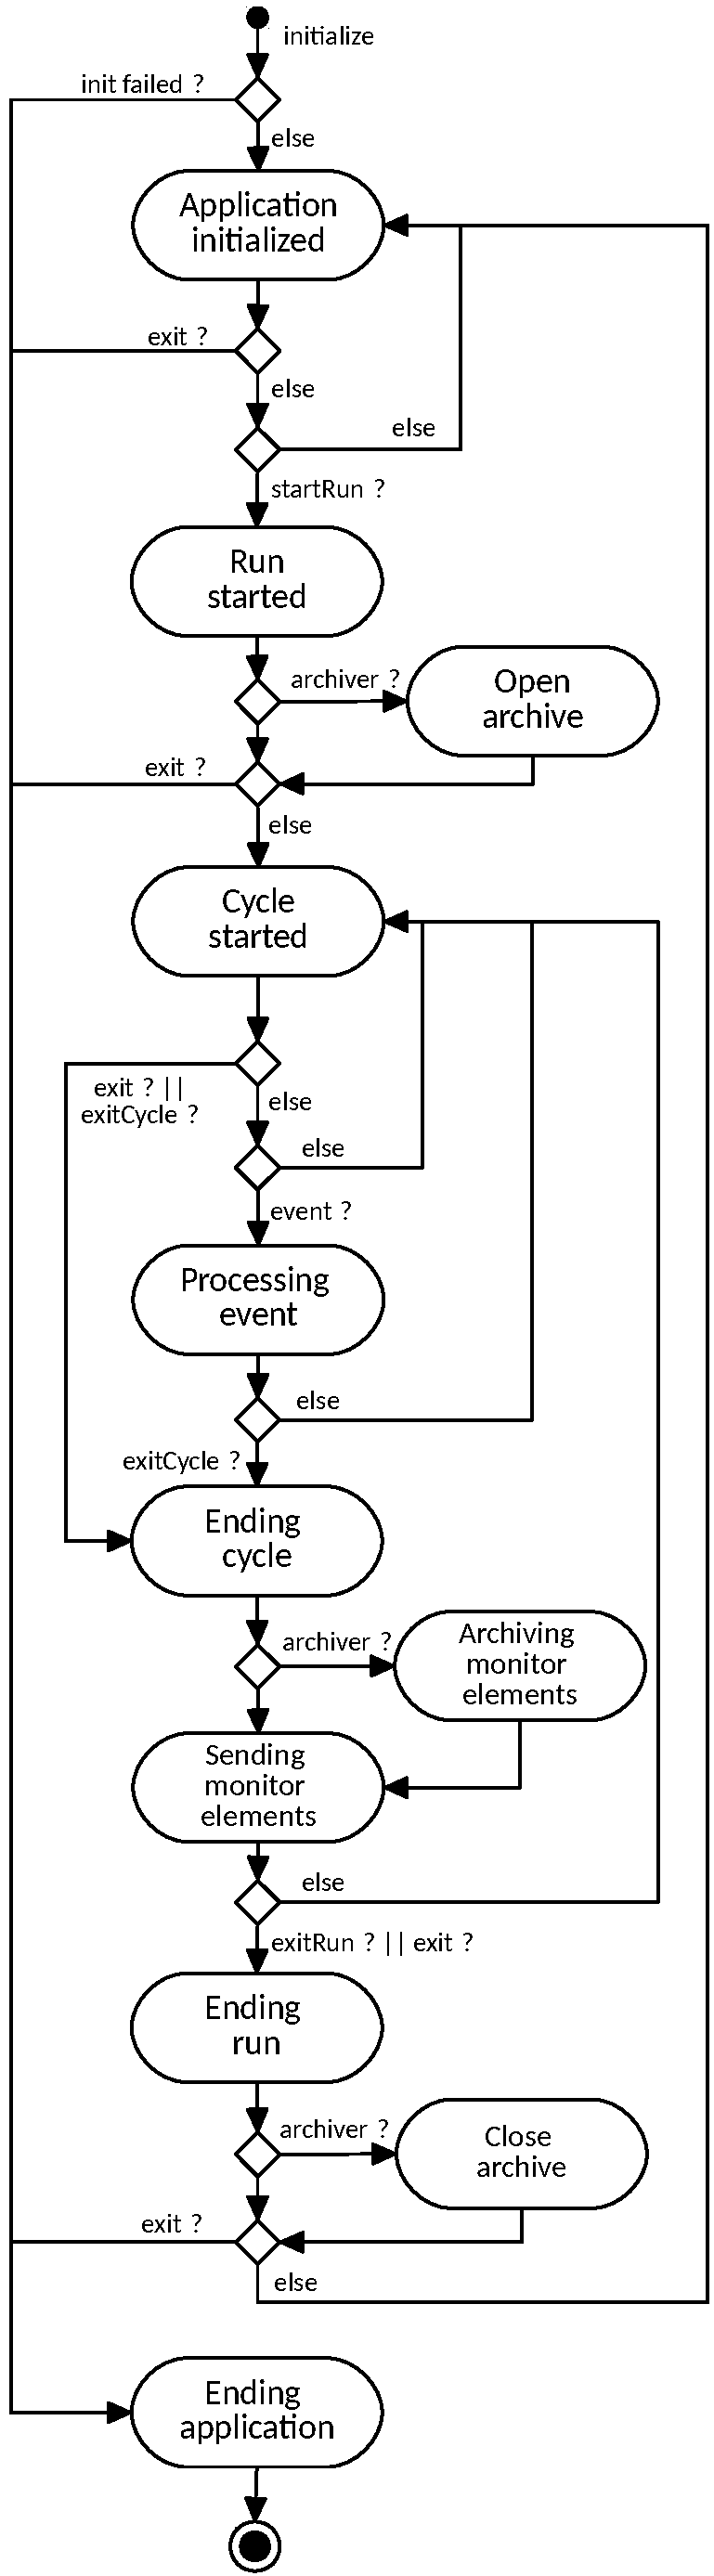
\includegraphics[width=0.65\linewidth]{figs/AnalysisModuleApplicatonWorkflowDiagram.pdf}
    \caption{\label{fig:DQMCycleSystem} Analysis module application workflow also showing cycle logic.}
  \end{center}
\end{figure}

\subsection{Remote control of the framework's application}
To deploy the framework for a target detector setup, multiple applications needs to be run (collectors, analysis modules, etc.) sometimes over a selection of hosts. There is then a need for an easy way of controlling them. \textit{Job control servers} serves this purpose. They are run as Linux daemons on every host involved in the deployment and each managing a set a processes that can be steered remotely from a client interface. Process information, such as process status or environment variables, can be permanently accessed from the client interface for process monitoring purpose.

%~~~~~~~~~~~~~~~~~~~~~~~~~~~~~~~~~~~~~~~~~~~~~~~~~~~~~~~~~~~~~~~~%
%~~~~~~~~~~~~~~~~~~~~~~~~~~~~~~~~~~~~~~~~~~~~~~~~~~~~~~~~~~~~~~~~%
\section{Graphical user interfaces (GUIs)}

\subsection{Monitoring GUI}

This graphical user interface implements a multiple access available monitor element collectors over the network. After the application start-up, the user can browse the monitor element collectors content and build selection of monitor element to draw. The main interface, as shown in Fig.~\ref{fig:DQMMainViz}, displays on the left the list of \textit{monitor element (ME)} the user selected has of interest at that time. These \textit{ME} can be displayed on the drawing section where a set of canvases are organized in a tab system. Every drawn \textit{ME} is interactive and can be manipulated according to the frontend used to display them (only ROOT~\cite{ROOT} for now.)
\begin{figure}[p]
  \begin{center}
    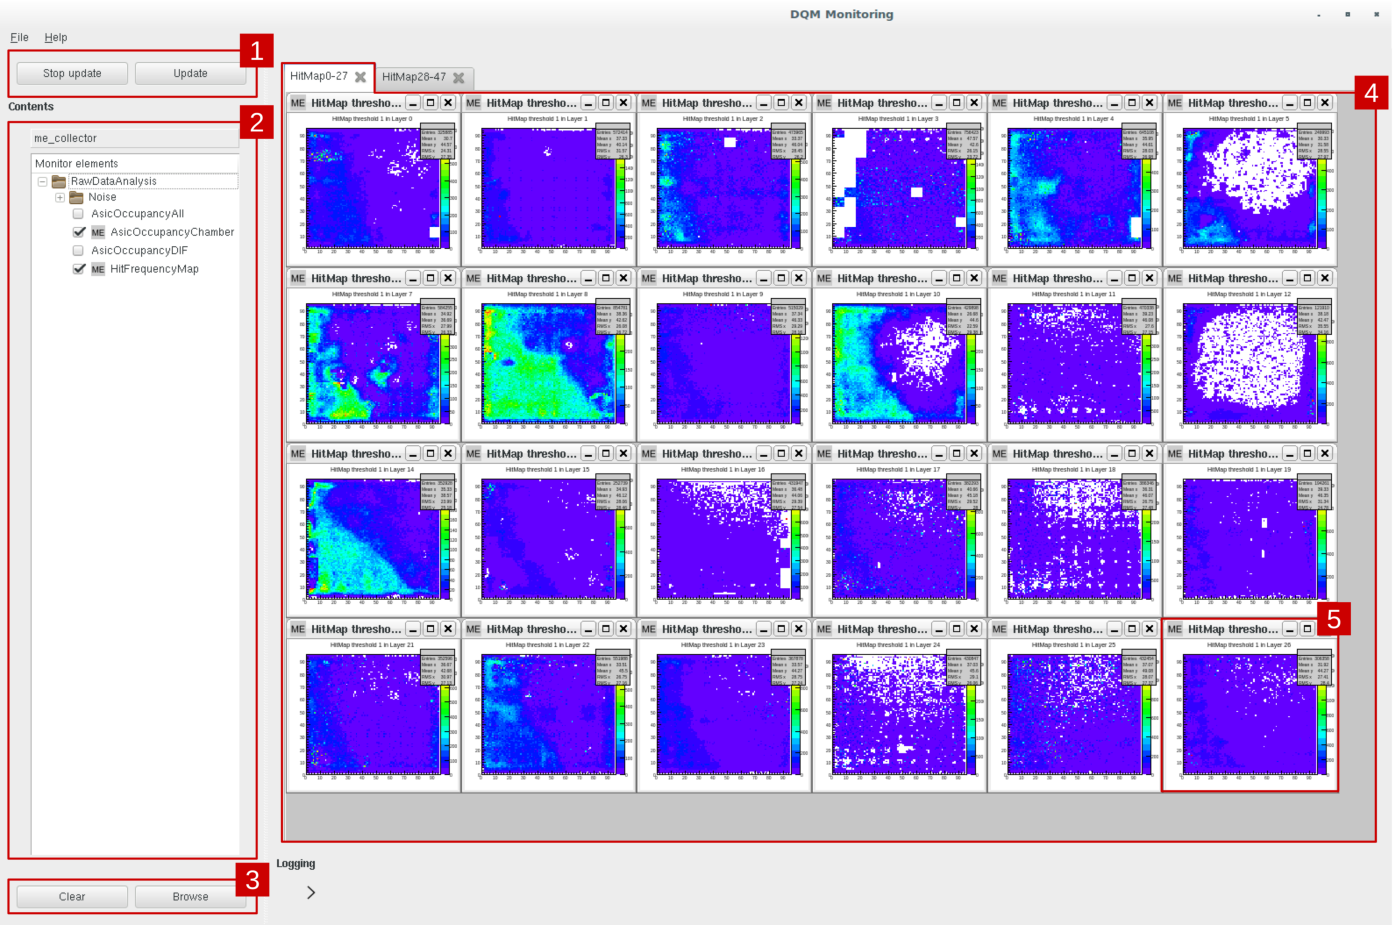
\includegraphics[width=0.8\linewidth]{figs/MaintInterfaceGUI.pdf}
    \caption{\label{fig:DQMMainViz} {\color{red}Put figures in One column page at the end}
    Main graphical interface of the framework.
    1. Option for manual/auto update.
    2. Monitor Elements (ME) organized in a tree-like structure
    3. List of displayed ME customizable via dedicated GUI with available ME (coming from analysis modules currently loaded)
    4. Drawing section for ME, can be organized in multiple tabs.
    5. Drawn ME are interactive, here ROOT[3] object that can be manipulated (zoom, change scale, fit, save, etc.)
    }
  \end{center}
\end{figure}

\subsection{Job control GUI}

This GUI is a graphic implementation of multiple job server clients. Processes can be loaded from a JSON file and added to the central process table as shown on Fig.~\ref{fig:JobControlGUI}. User can start/stop application on the different hosts using the interface but also monitor the process status by querying single process status or starting an automatic timer that refreshes the interface automatically. When starting a process on a host, a log file is created on the job control server and can be accessed at any time form this graphical user interface.

\begin{figure}[p]
  \begin{center}
    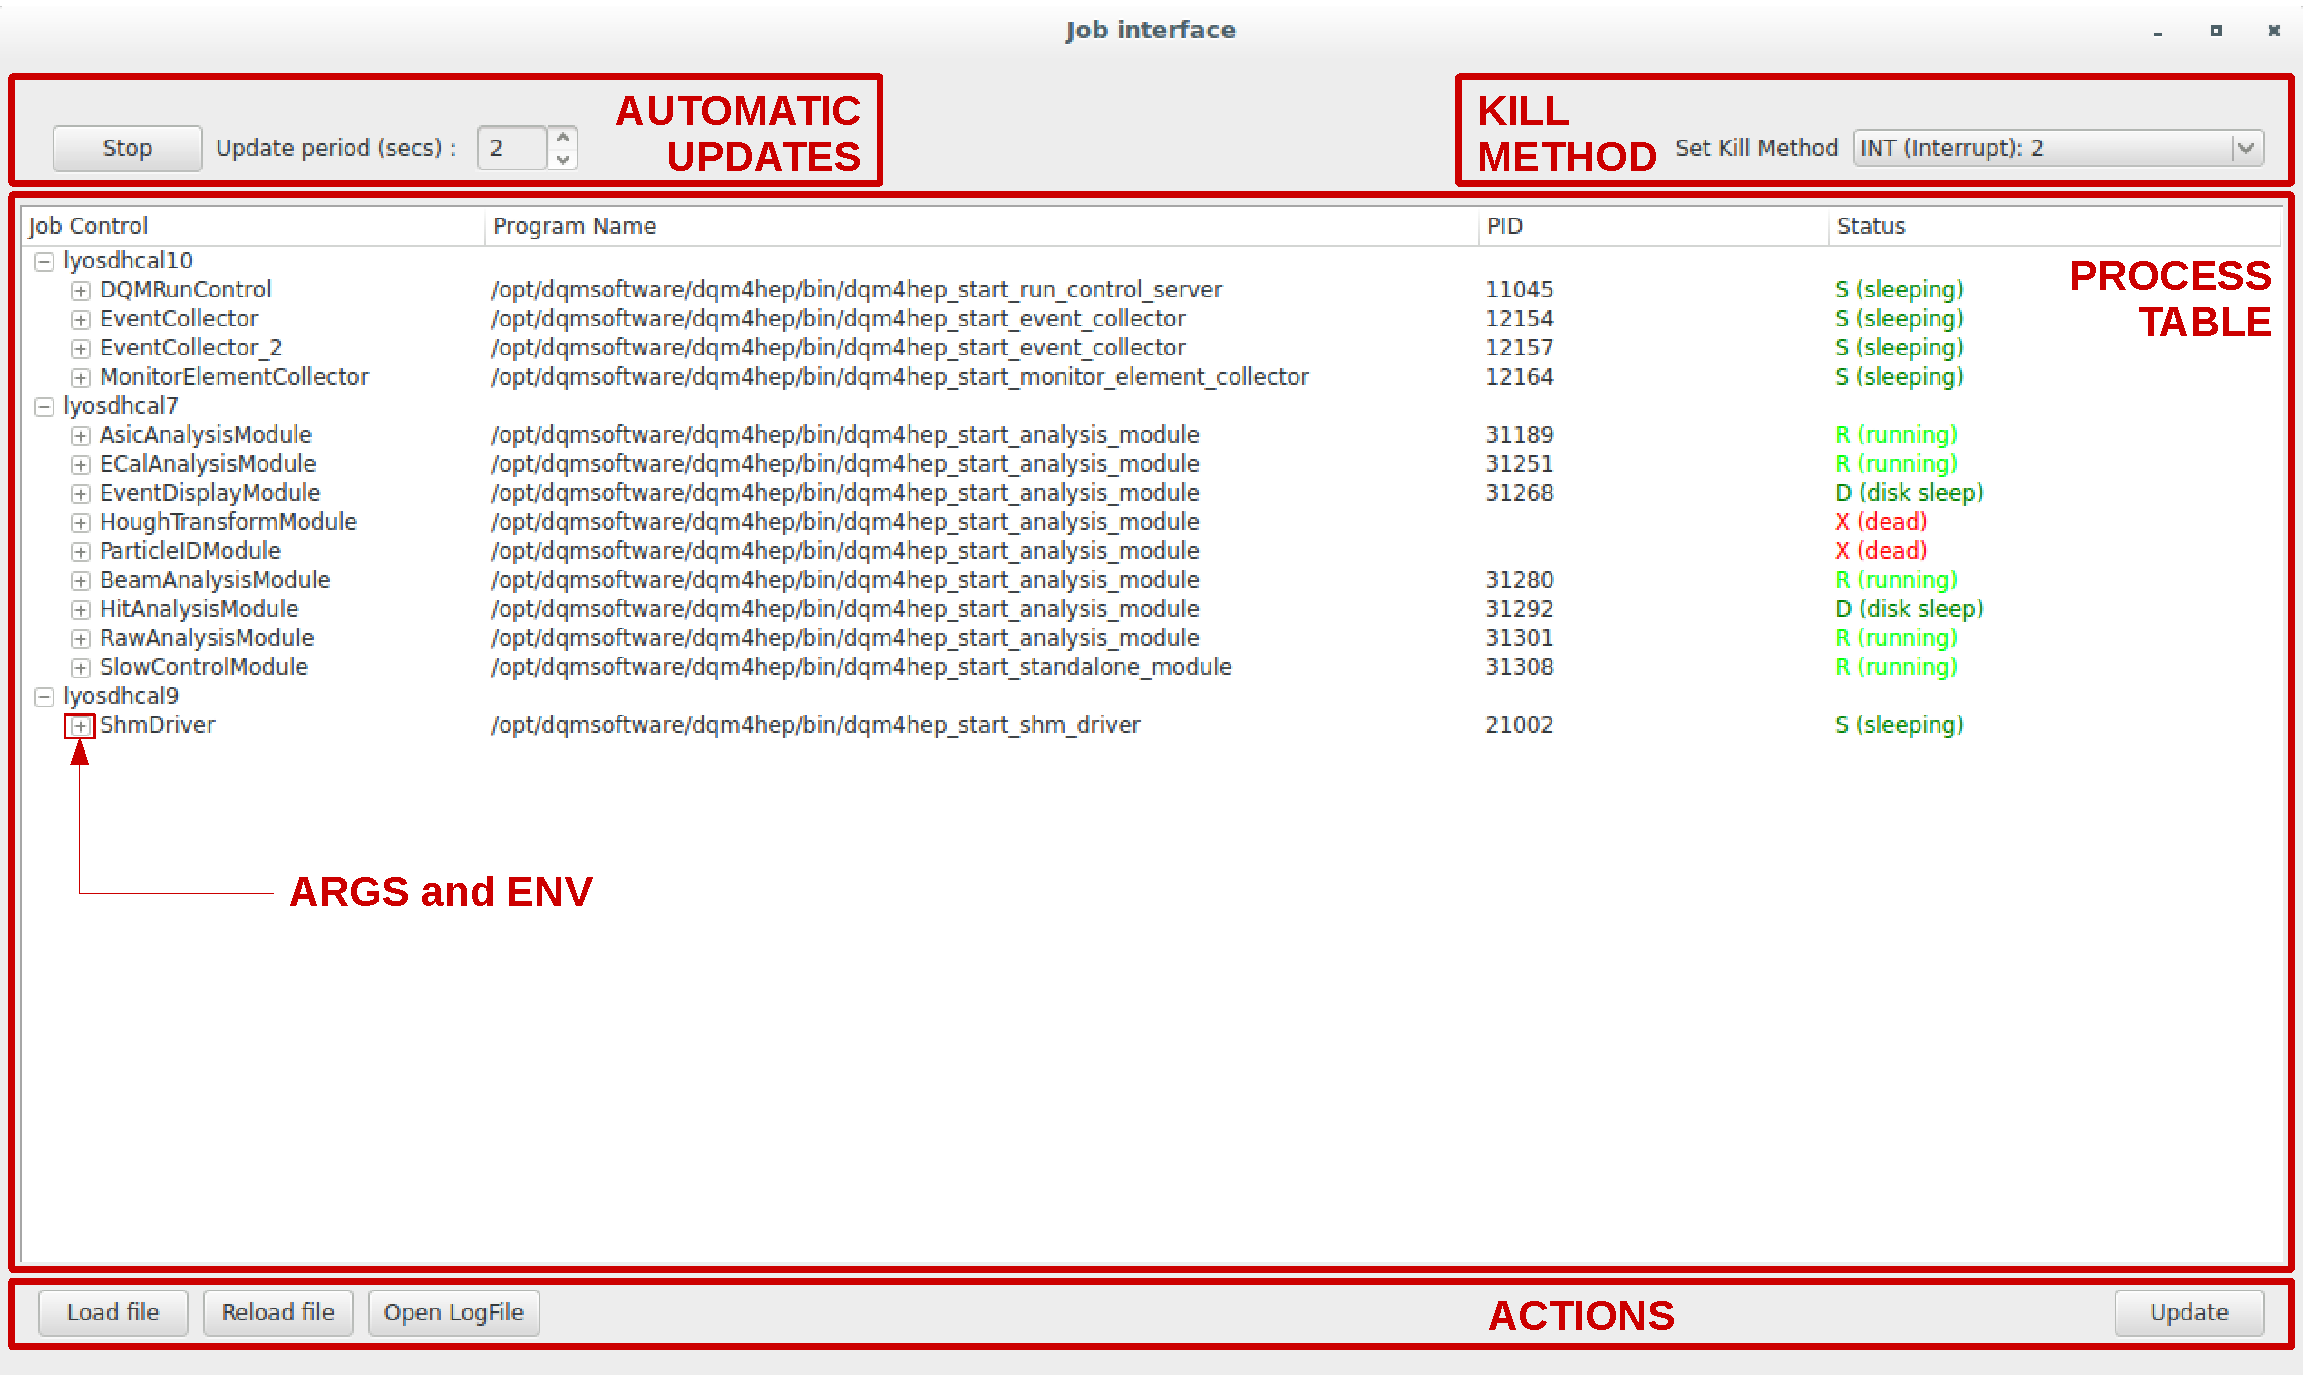
\includegraphics[width=0.95\linewidth]{figs/JobControlGui.pdf}
    \caption{\label{fig:JobControlGUI} GUI for the job interface. Applications are ordered by host}
  \end{center}
\end{figure}

\subsection{Run control GUI}

This GUI implements a graphical client interface to a run control server. The run control server application is mostly designed to receive start and stop run signals from the DAQ and dispatch it to all listening DQM applications. Moreover, the GUI implementation can also steers these signals and display the current run status in case the deployment is run without a DAQ, in a test mode.

%~~~~~~~~~~~~~~~~~~~~~~~~~~~~~~~~~~~~~~~~~~~~~~~~~~~~~~~~~~~~~~~~%
%~~~~~~~~~~~~~~~~~~~~~~~~~~~~~~~~~~~~~~~~~~~~~~~~~~~~~~~~~~~~~~~~%
\section{Implementation}

As the framework was developed within the CALICE-SDHCAL\footnote{Semi Digital Hadronic CALorimeter} Collaboration, a dedicated implementation has been produced in parallel for this prototype. This implementation is based on the LCIO~\cite{LCIO} Event Data Model, and provides interfaces for event type definition and serialization in this format.


Concerning the link to the DAQ system, the run control commands are received through HTTP POST and dispatch to the rest of the framework with DIM. The event building is based on \textit{levbdim}, the event builder used by the DAQ system for first level data reconstruction. In the SDHCAL case, the DAQ dumps the raw data coming from the detector to a shared memory (\textit{shm}) space as data sources buffers. The framework pulls a copy of these buffers and converts them to a LCIO format suitable for analysis with the online event builder implemented as plugins.

As the LCIO EDM contains multiple data structures for different levels of data reconstruction, converters are provided to pass from one such structure to the other. This gives the ability to use off-line analysis into the monitoring system, leading to a better assessment of the overall data quality.

For testing purposes, an offline data reader is also included in this implementation. This allows us to run the framework without a DAQ system running, especially handy to configure it properly in advance of a test beam campaign. To keep conditions as close as possible to a real setup, it can be configured to simulate the timing structure of the raw data.

At the online analysis level, many analysis and standalone modules were developed. Along with the DQM4HEP framework development, we gathered already existing analysis code for this experiment and adapted it to plug it in the framework. Some of these modules are briefly discussed hereafter. 

The \textit{Event Display} module allows for 2D and 3D visualization of the data in the detector. A 70GeV pion interacting in the SDHCAL as seen in the monitoring system is displayed in Fig.~\ref{fig:DQMEventDisplay}. A slow control module monitors the high voltages and current in every part of the detector together with the ambient temperature and pressure. This module is critical as too high value of current or high voltage can irremediably compromise the detector working order and thus the data quality. A module was in charge of evaluating the efficiency for each of the 50 chambers of the SDHCAL. Another module was developed to monitor informations related to the beam configuration such as rates of incoming particles as seen by the detector. 

One of these campaigns was dedicated to testing data taking in combination with the CALICE-SiWEcal\footnote{Silicon (W)Tungsten Electronic calorimeter)} experiment. Thus, we also developed some analysis dedicated to monitoring parts of this prototype, displaying i.e, ADC counter maps for each detector layer.

\begin{figure}[p]
  \begin{center}
    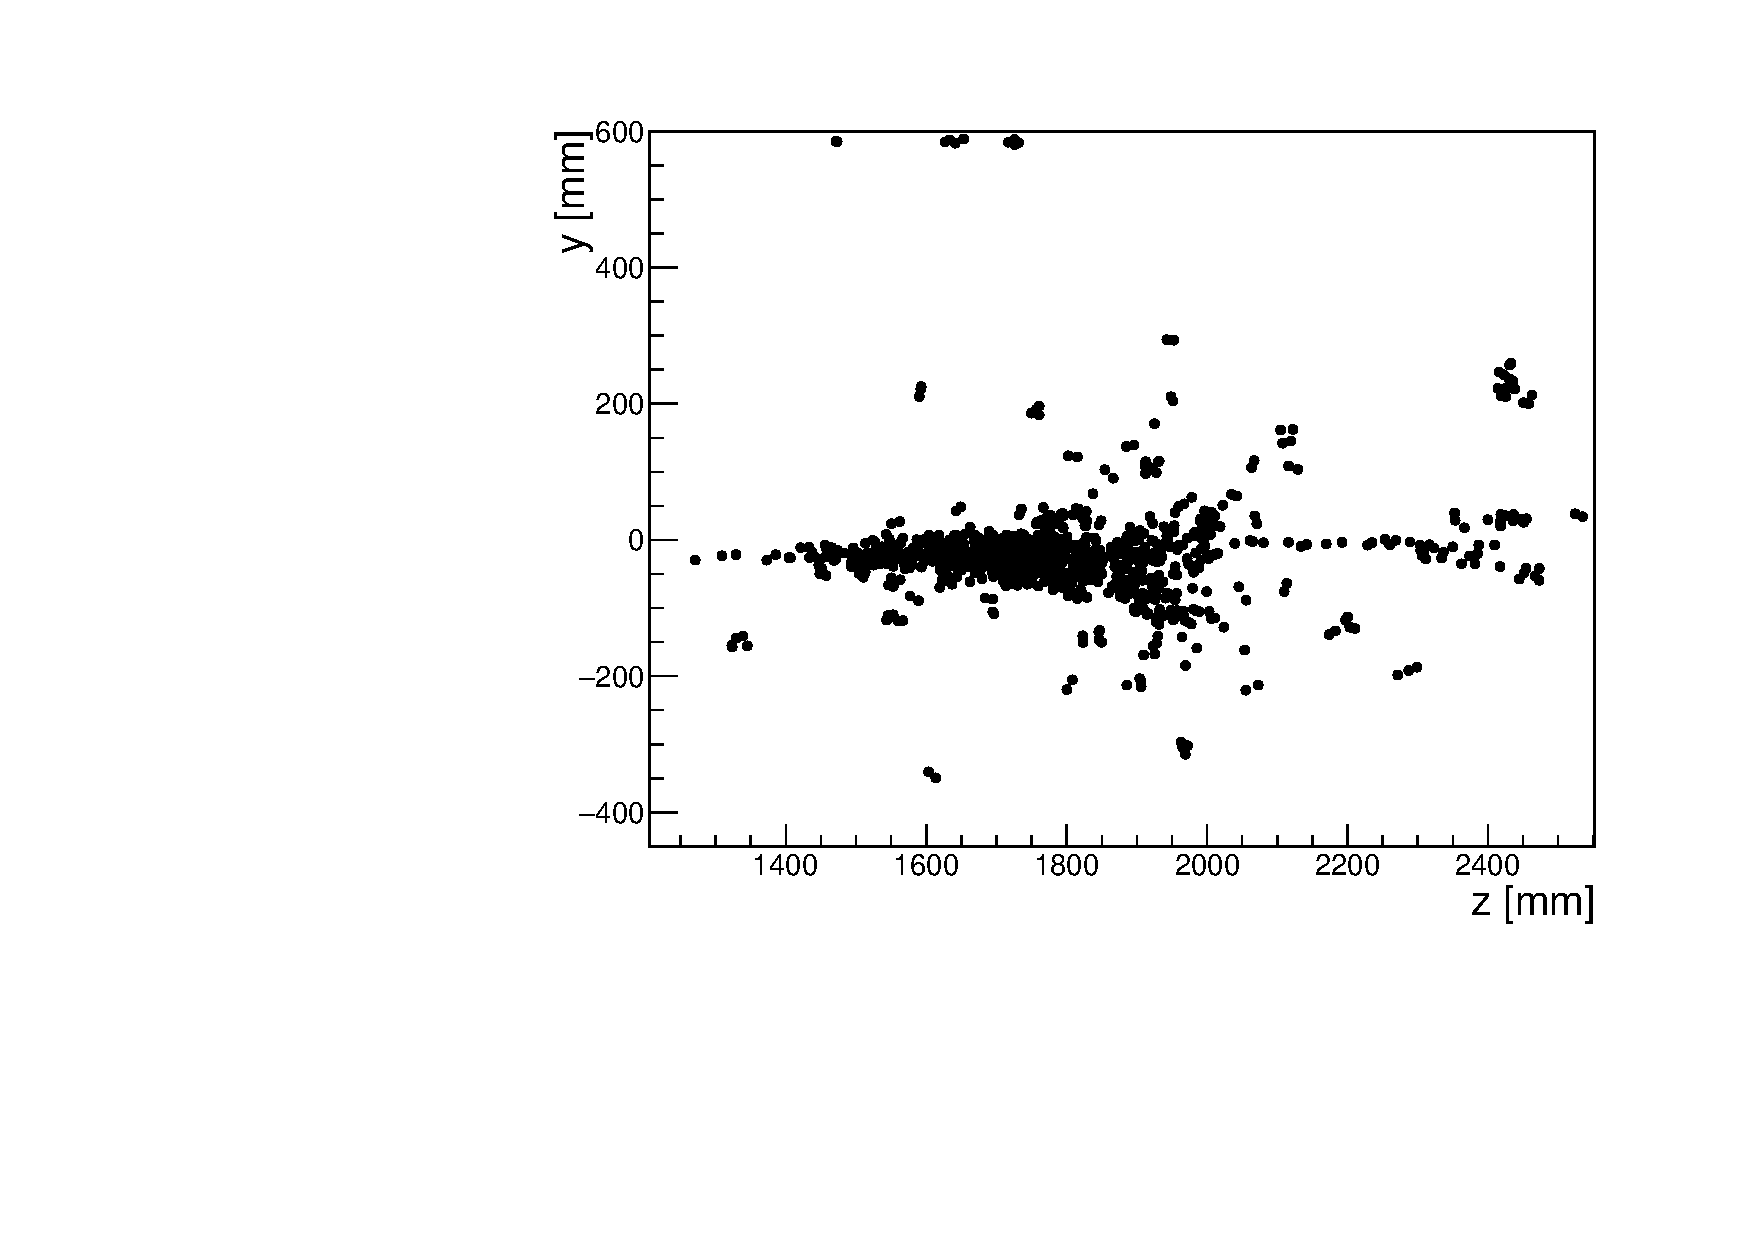
\includegraphics[width=0.8\linewidth]{figs/DQM_SDHCAL_Shower_pi-_70GeV_I732792.pdf}
    \caption{\label{fig:DQMEventDisplay} 2D Transversale view of a 70GeV pion in the SDHCAL prototype}
  \end{center}
\end{figure}

With this deployment, shifters were able to quickly spot and correct for multiple problems including, but not limited to, bad gas circulation, undesirably noisy electronics, wrong beam configuration, etc...

%~~~~~~~~~~~~~~~~~~~~~~~~~~~~~~~~~~~~~~~~~~~~~~~~~~~~~~~~~~~~~~~~%
%~~~~~~~~~~~~~~~~~~~~~~~~~~~~~~~~~~~~~~~~~~~~~~~~~~~~~~~~~~~~~~~~%
\section{Conclusion}
In light of the critical importance of a tool to quickly detect problems and ensure a good data quality, a new generic framework for Data Quality Monitoring systems has been created, integrating full flexibility across experiment set-up.

Contrary to most systems available for High Energy Physics up to now, it is not tied to a given Event Data Model. All the tools needed to develop a specific implementation depending on specificities of the experiment, such as DAQ and serialization interface, data format and detector analysis, are provided within the framework.
The whole system is written in c++11 with Qt~\cite{QT} libraries for the GUI.

The whole framework was tested both with offline and online setup dedicated to the SDHCAL prototype. The online configuration was used during two test beam campaigns at CERN, totalling three weeks. One of these campaign was dedicated to a combined test with the CALICE-SiWEcal, for which online analysis were also developed.

A dedicated implementation for the CALICE SDHCAL and SiWECal prototypes has been developed in parallel. It was tested with success both with online and offline data during two test beam campaigns.


% needed in second column of first page if using \IEEEpubid
%\IEEEpubidadjcol

% An example of a floating figure using the graphicx package.
% Note that \label must occur AFTER (or within) \caption.
% For figures, \caption should occur after the \includegraphics.
% Note that IEEEtran v1.7 and later has special internal code that
% is designed to preserve the operation of \label within \caption
% even when the captionsoff option is in effect. However, because
% of issues like this, it may be the safest practice to put all your
% \label just after \caption rather than within \caption{}.
%
% Reminder: the "draftcls" or "draftclsnofoot", not "draft", class
% option should be used if it is desired that the figures are to be
% displayed while in draft mode.
%
%\begin{figure}[!t]
%\centering
%\includegraphics[width=2.5in]{myfigure}
% where an .eps filename suffix will be assumed under latex,
% and a .pdf suffix will be assumed for pdflatex; or what has been declared
% via \DeclareGraphicsExtensions.
%\caption{Simulation Results}
%\label{fig_sim}
%\end{figure}

% Note that IEEE typically puts floats only at the top, even when this
% results in a large percentage of a column being occupied by floats.


% An example of a double column floating figure using two subfigures.
% (The subfig.sty package must be loaded for this to work.)
% The subfigure \label commands are set within each subfloat command, the
% \label for the overall figure must come after \caption.
% \hfil must be used as a separator to get equal spacing.
% The subfigure.sty package works much the same way, except \subfigure is
% used instead of \subfloat.
%
%\begin{figure*}[!t]
%\centerline{\subfloat[Case I]\includegraphics[width=2.5in]{subfigcase1}%
%\label{fig_first_case}}
%\hfil
%\subfloat[Case II]{\includegraphics[width=2.5in]{subfigcase2}%
%\label{fig_second_case}}}
%\caption{Simulation results}
%\label{fig_sim}
%\end{figure*}
%
% Note that often IEEE papers with subfigures do not employ subfigure
% captions (using the optional argument to \subfloat), but instead will
% reference/describe all of them (a), (b), etc., within the main caption.


% An example of a floating table. Note that, for IEEE style tables, the
% \caption command should come BEFORE the table. Table text will default to
% \footnotesize as IEEE normally uses this smaller font for tables.
% The \label must come after \caption as always.
%
%\begin{table}[!t]
%% increase table row spacing, adjust to taste
%\renewcommand{\arraystretch}{1.3}
% if using array.sty, it might be a good idea to tweak the value of
% \extrarowheight as needed to properly center the text within the cells
%\caption{An Example of a Table}
%\label{table_example}
%\centering
%% Some packages, such as MDW tools, offer better commands for making tables
%% than the plain LaTeX2e tabular which is used here.
%\begin{tabular}{|c||c|}
%\hline
%One & Two\\
%\hline
%Three & Four\\
%\hline
%\end{tabular}
%\end{table}


% Note that IEEE does not put floats in the very first column - or typically
% anywhere on the first page for that matter. Also, in-text middle ("here")
% positioning is not used. Most IEEE journals use top floats exclusively.
% Note that, LaTeX2e, unlike IEEE journals, places footnotes above bottom
% floats. This can be corrected via the \fnbelowfloat command of the
% stfloats package.


% if have a single appendix:
%\appendix[Proof of the Zonklar Equations]
% or
%\appendix  % for no appendix heading
% do not use \section anymore after \appendix, only \section*
% is possibly needed

% use appendices with more than one appendix
% then use \section to start each appendix
% you must declare a \section before using any
% \subsection or using \label (\appendices by itself
% starts a section numbered zero.)
%

%
% \appendices
% \section{Proof of the First Zonklar Equation}
% \blindtext

% use section* for acknowledgement
\section*{Acknowledgment}

The authors would like to thank...NO ONE BUT THEMSELVES FOR ALL THIS HAAAAARWORK. Science, Bitch!


% Can use something like this to put references on a page
% by themselves when using endfloat and the captionsoff option.
\ifCLASSOPTIONcaptionsoff
  \newpage
\fi



% trigger a \newpage just before the given reference
% number - used to balance the columns on the last page
% adjust value as needed - may need to be readjusted if
% the document is modified later
%\IEEEtriggeratref{8}
% The "triggered" command can be changed if desired:
%\IEEEtriggercmd{\enlargethispage{-5in}}

% references section

% can use a bibliography generated by BibTeX as a .bbl file
% BibTeX documentation can be easily obtained at:
% http://www.ctan.org/tex-archive/biblio/bibtex/contrib/doc/
% The IEEEtran BibTeX style support page is at:
% http://www.michaelshell.org/tex/ieeetran/bibtex/
%\bibliographystyle{IEEEtran}
% argument is your BibTeX string definitions and bibliography database(s)
%\bibliography{IEEEabrv,../bib/paper}
%
% <OR> manually copy in the resultant .bbl file
% set second argument of \begin to the number of references
% (used to reserve space for the reference number labels box)

\begin{thebibliography}{1}

\bibitem{LCIO}
% Frank Gaede, \emph{\tt lcio.desy.de}, 2016.
S. Aplin et al., "LCIO: A persistency framework and event data model for HEP", \emph{Nuclear Science Symp. and Medical Imaging Conf. (NSS/MIC), 2012 IEEE}, Anaheim, CA, 2012, pp. 2075-2079.

\bibitem{DIM}
C. Gaspar et al., "DIM, a Portable, Light Weight Package for Information Publishing, Data Transfer and Inter-process Communication" presented at the \emph{Int. Conf. Computing in High Energy and Nuclear Physics}, Padova, Italy, 2000)

\bibitem{MONGOOSE}
Michael J Hammel, "Mongoose: an embeddable web server in C", \emph{Linux Journal}, 2010, pp. 192

\bibitem{QT}
% J. Blanchette and M. Summerfield
Qt Company, \emph{\tt http://www.qt.io}, v4.7, 2016.

\bibitem{ROOT}
Rene Brun and Fons Rademakers, "ROOT - An Object Oriented Data Analysis Framework", \emph{Nucl. Inst. \& Meth. in Phys. Res. A 389}, 1997, pp. 81-86. Available: http://root.cern.ch/

\bibitem{MARLIN}
F. Gaede,  "Marlin and LCCD: Software tools for the ILC", \emph{Nucl. Inst. \& Meth. A559}, 2006, pp. 177-180

\end{thebibliography}


% biography section
%
% If you have an EPS/PDF photo (graphicx package needed) extra braces are
% needed around the contents of the optional argument to biography to prevent
% the LaTeX parser from getting confused when it sees the complicated
% \includegraphics command within an optional argument. (You could create
% your own custom macro containing the \includegraphics command to make things
% simpler here.)
%\begin{biography}[{\includegraphics[width=1in,height=1.25in,clip,keepaspectratio]{mshell}}]{Michael Shell}
% or if you just want to reserve a space for a photo:

\begin{IEEEbiography}[{\includegraphics[width=1in,height=1.25in,clip,keepaspectratio]{picture}}]{John Doe}
\blindtext
\end{IEEEbiography}



% You can push biographies down or up by placing
% a \vfill before or after them. The appropriate
% use of \vfill depends on what kind of text is
% on the last page and whether or not the columns
% are being equalized.

%\vfill

% Can be used to pull up biographies so that the bottom of the last one
% is flush with the other column.
%\enlargethispage{-5in}




% that's all folks
\end{document}
